\documentclass[12pt]{article}
\usepackage{graphicx}
\usepackage{listings}
\begin{document}

\begin{titlepage}
\begin{center} 
 \textsc{\large Facultatea Calculatoare, Informatica si Microelectronica}\\[0.5cm]
\textsc{\large Universitatea Tehnica a Moldovei}\\[1.2cm] 
\vspace{25 mm}

\textsc{\Large Medii Interactive de Dezvoltare a Produselor Soft}\\[0.5cm] 
\textsc{\large Lucrarea de laborator\#1}\\[0.5cm] \newcommand{\HRule}{\rule{\linewidth}{0.5mm}} 
  \vspace{10 mm}
  \HRule \\[0.4cm]
  { \LARGE \bfseries Mediul integrat C++ Builder  }\\[0.4cm] 
  \HRule \\[1.5cm]
      \vspace{30mm}

      \begin{minipage}{0.4\textwidth}
      \begin{flushleft} \large
      \emph{Autor:}\\
      Alexandr \textsc{Ialticenco}
      \end{flushleft}
      \end{minipage}
      ~
      \begin{minipage}{0.4\textwidth}
      \begin{flushright} \large
      \emph{lector asistent:} \\
      Irina \textsc{Cojanu} \\ 
      \emph{lector superior:} \\
      Svetlana \textsc{Cojocaru} 
      \end{flushright}
      \end{minipage}\\[4cm]

      \vspace{5 mm}

      \vfill
      \end{center}
      
\end{titlepage}

\section*{Obiectivele lucrarii}
\begin{itemize}
\item Insuşirea modului de utilizare a celor mai importante componente ale mediului integrat C++ BUILDER . Realizarea unui program simplu care utilizeaza componente de tip TButton, TEdit, Tlabel, RadioButton  etc.  
\item Insuşirea modului de utilizare a componentei VCL TTimer. Insuşirea modului de utilizare a functiilor de lucru cu timpul sistem. Realizarea unor aplicatii de gestionare a resursei timp.
\item Insuşirea modului de utilizare a componentelor VCL  TPaintBox si TPanel. Însuşirea modului de utilizare a principalelor functii grafice ale mediului C++BUILDER . Realizarea unor elemente pentru  afisarea grafica a informatiei (diagrama si bargraf).
\end{itemize}

\section* {Sarcina lucrarii}
\begin{itemize}
\item Vor fi examinate toate componentele prezentate in indicatii teoretice;
\item Se modifica Project1.cpp ca sa se obtina forma de mai jos\\
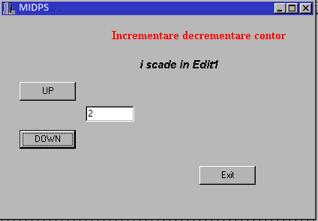
\includegraphics[width=12.5cm]{images/1}
\item Se  elaboreaza  un program pentru realizarea unui cronometru.
Se vor utiliza următoarele obiecte, evidentiate în figura de mai jos:
\\
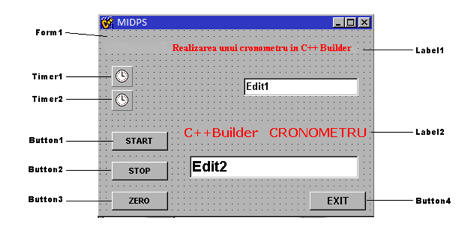
\includegraphics[width=16cm]{images/2}
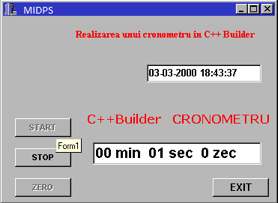
\includegraphics[width=12.5cm]{images/3}\\
\item Se  elaboreaza  un program pentru realizarea a doua elemente de afisare (bargraf si diagramă cu avans continuu) pentru care forma arată ca în figura de mai jos pe care sunt dispuse următoarele obiecte:\\
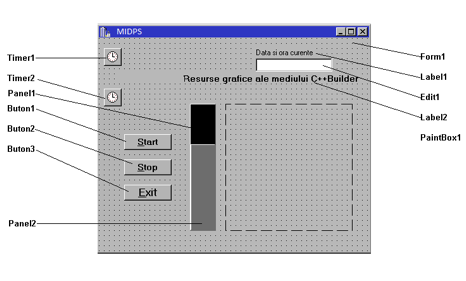
\includegraphics[width=12.5cm]{images/4}\\
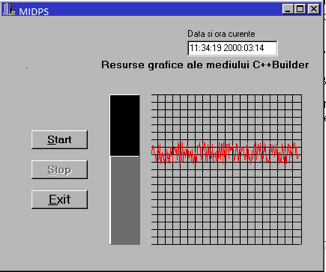
\includegraphics[width=10.5cm]{images/5}
\end{itemize}
\section {Incrementator}
\subsection{Listingul}
\textbf{Modul GUI va fi encapsulat in clasa Form1.}
\begin{lstlisting}
//---------


#include <vcl.h>

#pragma hdrstop



#include "Unit1.h"

//---------
#pragma package(smart_init)

#pragma resource "*.dfm"

TForm1 *Form1;

int i;

//-------
__fastcall TForm1::TForm1(TComponent* Owner)

        : TForm(Owner)

{

}

//-------



void __fastcall TForm1::Button3Click(TObject *Sender)

{

Close();        

}

//--------

void __fastcall TForm1::FormCreate(TObject *Sender)

{

i = 0;

Edit1->Text = i;

}

//--------
void __fastcall TForm1::Button1Click(TObject *Sender)

{

Edit1->Text = ++i;

}

//---------

void __fastcall TForm1::Button2Click(TObject *Sender)

{

Edit1->Text = --i;

}

//---------

\end{lstlisting}
\subsection{Screenshot-ul aplicatiei}
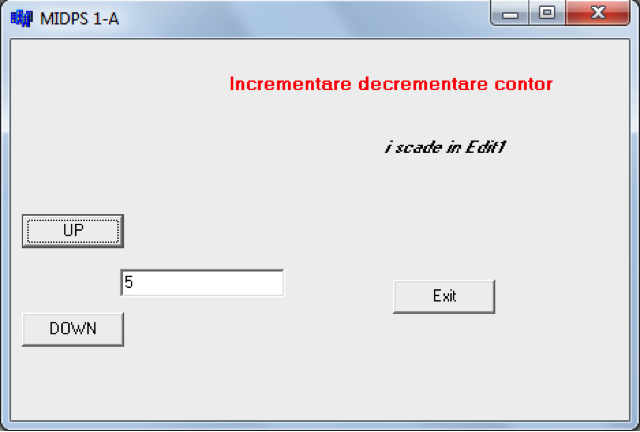
\includegraphics[width=10.5cm]{images/6}

\section{Cronometru}
\subsection{Listingul}
\begin{lstlisting}
//---------



#include <vcl.h>

#include <stdio.h>

#pragma hdrstop 

#include "Unit1.h"

//---------

#pragma package(smart_init)

#pragma resource "*.dfm"

#include "dos.h"

TForm1 *Form1;

struct time t;

struct date d;

int min, sec, zec;

//---------

__fastcall TForm1::TForm1(TComponent* Owner)

        : TForm(Owner)

{

}

//---------



void __fastcall TForm1::Timer1Timer(TObject *Sender)

{

char buf[20];

getdate(&d);

gettime(&t);

sprintf(buf,"%02d-%02d-%4d %02d:%02d:
%02d",d.da_day,d.da_mon,d.da_year,

t.ti_hour,t.ti_min,t.ti_sec);

Edit1->Text=(AnsiString)buf;

}

//---------

void __fastcall TForm1::Button1Click(TObject *Sender)

{

Timer2->Enabled = true;

Button2->Enabled = true;

Button1->Enabled = false;

Button3->Enabled = false;

}

//---------

void __fastcall TForm1::Timer2Timer(TObject *Sender)

{

zec += 1;

if (zec >= 10){

zec = 0;

sec ++;

}

if (sec>=60){

sec = 0;

min ++;

}

char buf[20];

sprintf(buf,"%02d min %02d sec %d zec",min,sec, zec);

Edit2->Text=(AnsiString)buf;

}

//---------

void __fastcall TForm1::Button2Click(TObject *Sender)

{

Timer2->Enabled = false;

Button1->Enabled = true;

Button3->Enabled = true;

Button2->Enabled = false;

}

//---------

void __fastcall TForm1::Button3Click(TObject *Sender)

{

min = sec = zec = 0;

char buf[20];

sprintf(buf,"%02d min %02d sec %d zec",min,sec, zec);

Edit2->Text=(AnsiString)buf;

}

//---------

void __fastcall TForm1::Button4Click(TObject *Sender)

{

Close();        

}

//---------



void __fastcall TForm1::FormCreate(TObject *Sender)

{

char buf[20];

getdate(&d);

gettime(&t);

sprintf(buf,"%02d-%02d-%4d %02d:
%02d:%02d",
d.da_day,d.da_mon,
d.da_year,

t.ti_hour,t.ti_min,t.ti_sec);

Edit1->Text=(AnsiString)buf;

}
	
\end{lstlisting}
\subsection{Screenshot-ul aplicatiei}
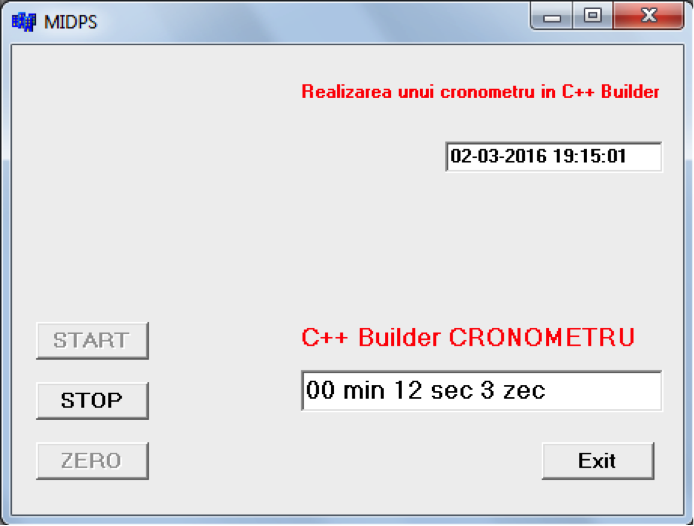
\includegraphics[width=10.5cm]{images/7}
\section{Bargraful}
\subsection{Listingul}
\begin{lstlisting}
	Codul sursa:

//---------


#include <vcl.h>

#pragma hdrstop

#include <stdio.h>

#include "Unit1.h"

#include "dos.h"

//---------

#pragma package(smart_init)

#pragma resource "*.dfm"

TForm1 *Form1;

struct time t;

struct date d;

TRect rect;

int nextY, next2Y, nextP;

bool first;

//---------

__fastcall TForm1::TForm1(TComponent* Owner)

        : TForm(Owner)

{

}

//---------



void __fastcall TForm1::Button3Click(TObject *Sender)

{

Close();        

}

//---------



void __fastcall TForm1::Button1Click(TObject *Sender)

{

Button1->Enabled = false;

Button2->Enabled = true;

Timer2->Enabled = true;

first = true;

rect.Left = 0;

rect.Right = 300;

rect.top = 0;

rect.Bottom = 300;

}

//---------



void __fastcall TForm1::Button2Click(TObject *Sender)

{

Button1->Enabled = true;

Button2->Enabled = false;

Timer2->Enabled = false;

}

//---------

void __fastcall TForm1::Timer1Timer(TObject *Sender)

{

char buf[20];

getdate(&d);

gettime(&t);

sprintf(buf,"%02d-%02d-%4d %02d:
%02d:%02d",d.da_day,d.da_mon,d.da_year,

t.ti_hour,t.ti_min,t.ti_sec);

Edit1->Text=(AnsiString)buf;

}

//---------

void cells(){



}

void __fastcall TForm1::Timer2Timer(TObject *Sender)

{

if (first){

nextP =  abs(rand()%100);

nextY = abs(rand()%100);

PaintBox1->Canvas->Pen->Color = clBlack;

for (int i =0; i<31; i++){

PaintBox1->Canvas->MoveTo(0,i*10);

PaintBox1->Canvas->LineTo(300,i*10);

}

for (int i =0; i<31; i++){

PaintBox1->Canvas->MoveTo(i*10,0);

PaintBox1->Canvas->LineTo(i*10,300);

}

first = false;

}

TRect rect2;

rect2.left = 0;

rect2.right = 300;

rect2.top = 0;

rect2.bottom = 300;

rect.left = -10;

rect.right = 290;

TRect rect3;

rect3.left = 290; 
rect3.right = 300; 
rect3.top = 0; 
rect3.bottom = 300;

PaintBox1->Canvas->FillRect(rect3);

PaintBox1->Canvas->MoveTo(290,0);

PaintBox1->Canvas->LineTo(290,300);

for (int i =0; i<31; i++){

PaintBox1->Canvas->MoveTo(290,i*10);

PaintBox1->Canvas->LineTo(300,i*10);

}

PaintBox1->Canvas->MoveTo(290,nextY+100);

PaintBox1->Canvas->Pen->Color = clRed;

nextY = next2Y;

PaintBox1->Canvas->LineTo(295,100+nextP);



PaintBox1->Canvas->LineTo(300,100+nextY);

PaintBox1->Canvas->CopyRect(rect,PaintBox1->Canvas, rect2);

PaintBox1->Canvas->Pen->Color = clBlack;



rect3.left = 290; rect3.right = 300; 
rect3.top = 0; rect3.bottom = 300;

PaintBox1->Canvas->FillRect(rect3);

PaintBox1->Canvas->MoveTo(290,0);

PaintBox1->Canvas->LineTo(290,300);



for (int i =0; i<31; i++){

PaintBox1->Canvas->MoveTo(290,i*10);

PaintBox1->Canvas->LineTo(300,i*10);

}



nextP =  abs(rand()%100);

PaintBox1->Canvas->Pen->Color = clRed;

next2Y = abs(rand()%100);

PaintBox1->Canvas->MoveTo(290,nextY+100);

PaintBox1->Canvas->LineTo(295,100+nextP);

PaintBox1->Canvas->LineTo(300,100+next2Y);

PaintBox1->Canvas->Pen->Color = clBlack;

PaintBox1->Canvas->MoveTo(300,0);

PaintBox1->Canvas->LineTo(300,300);

Panel2->Height = Panel1->Height*(nextP/100.0);

//PaintBox1->Canvas->FillRect(rect);

}

//---------



void __fastcall TForm1::FormCreate(TObject *Sender)

{

char buf[20];

getdate(&d);

gettime(&t);

sprintf(buf,"%02d-%02d-%4d %02d:
%02d:%02d",d.da_day,d.da_mon,d.da_year,

t.ti_hour,t.ti_min,t.ti_sec);

Edit1->Text=(AnsiString)buf;        

}

//---------
\end{lstlisting}
\subsection{Screenshot-ul aplicatiei}
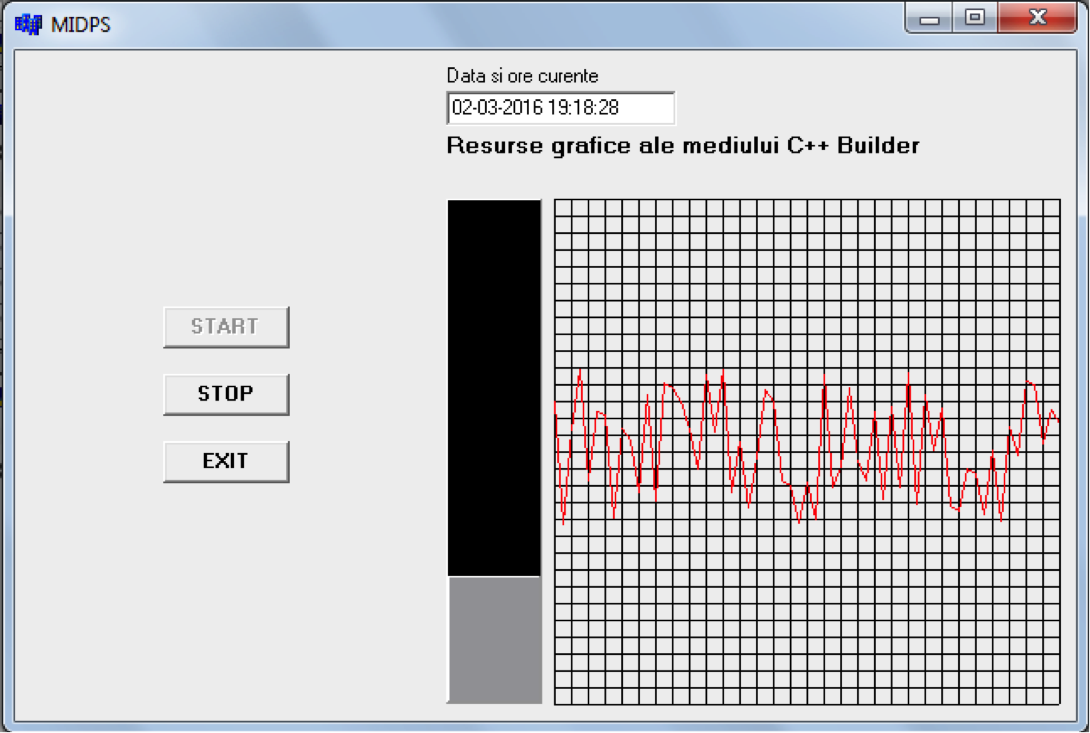
\includegraphics[width=10.5cm]{images/8}
\section*{Concluzii}
In cadrul acestei lucrari de laborator am studiat principiile si modul de utilizare a celor mai importante componente ale mediului integrat C++ Builder așa ca TButton, TEdit, TTimer, TPaintBox si etc. Bazand pe cunoștințele obtinute am reusit sa realizez trei aplicatii Windows cu interfata grafica, functionalul carora include nu doar interactiunea grafică dintre utilizator si aplicatia cat si gestionarea resursei de timp si afisarea grafica a informatiei (prin intermediul diagramelor si bargrafelor). Experiența si cunostințele obtinute pe parcursul indeplinirii lucrării de laborator vor fi utile în viitor si pot fi aplicate pentru realizarea proiectelor diferite.
\section*{Bibliografie}
\begin{enumerate}
\item http://www.functionx.com/cppbcb/ - \textbf{C++ Builder Programming}
\end{enumerate}





\end{document}